\chapter{How a node joins the system}
\label{chapter.join}
\svnrev{r1370}

After starting a new \scalaris{}-System as described in
Section~\sieheref{sec.boot}, ten additional local nodes can be started
by typing \code{api_vm:add_nodes(10)} in the Erlang-Shell that is
opened during startup~\footnote{Increase the log level to {\tt info} to get
more detailed startup logs. See Section~\sieheref{sec:logging}}.


\lstset{language=erlang}
\begin{lstlisting}
scalaris> ./bin/firstnode.sh 
[...]
(firstnode@csr-pc9)1> api_vm:add_nodes(10)
\end{lstlisting}

In the following we will trace what this function does in order to add
additional nodes to the system.
The function \erlfun{api\_vm}{add\_nodes}{pos\_integer()} is defined as follows.

\codesnippet{api_vm.erl}{api_vm:add_nodes}{../src/api_vm.erl}

It uses the \erlfun{admin}{add\_nodes}{/1} function to actually add the given
number of nodes and then waits for all nodes to successfully complete their
join phases.

\codesnippet{admin.erl}{admin:add_nodes}{../src/admin.erl}

The function \erlfun{admin}{add\_nodes}{/1} calls
\erlfun{admin}{add\_node}{[]} Count times. This function starts a new
child with the given options for the main supervisor \code{main_sup}.
In particular, it sets a random ID that is passed to the new node as its
suggested ID to join at.
To actually perform the start, the
function \erlfun{sup\_dht\_node}{start\_link}{/1} is called by the Erlang
supervisor mechanism. For more details on the OTP supervisor
mechanism see Chapter~18 of the Erlang book~\cite{erlang-book} or the
online documentation at
\url{http://www.erlang.org/doc/man/supervisor.html}.

\section{Supervisor-tree of a \scalaris{} node}

When a new Erlang VM with a \scalaris{} node is started, a
\erlmodule{sup\_scalaris} supervisor is started that creates further
workers and supervisors according to the following scheme
(processes starting order: left to right, top to bottom):

\begin{center}
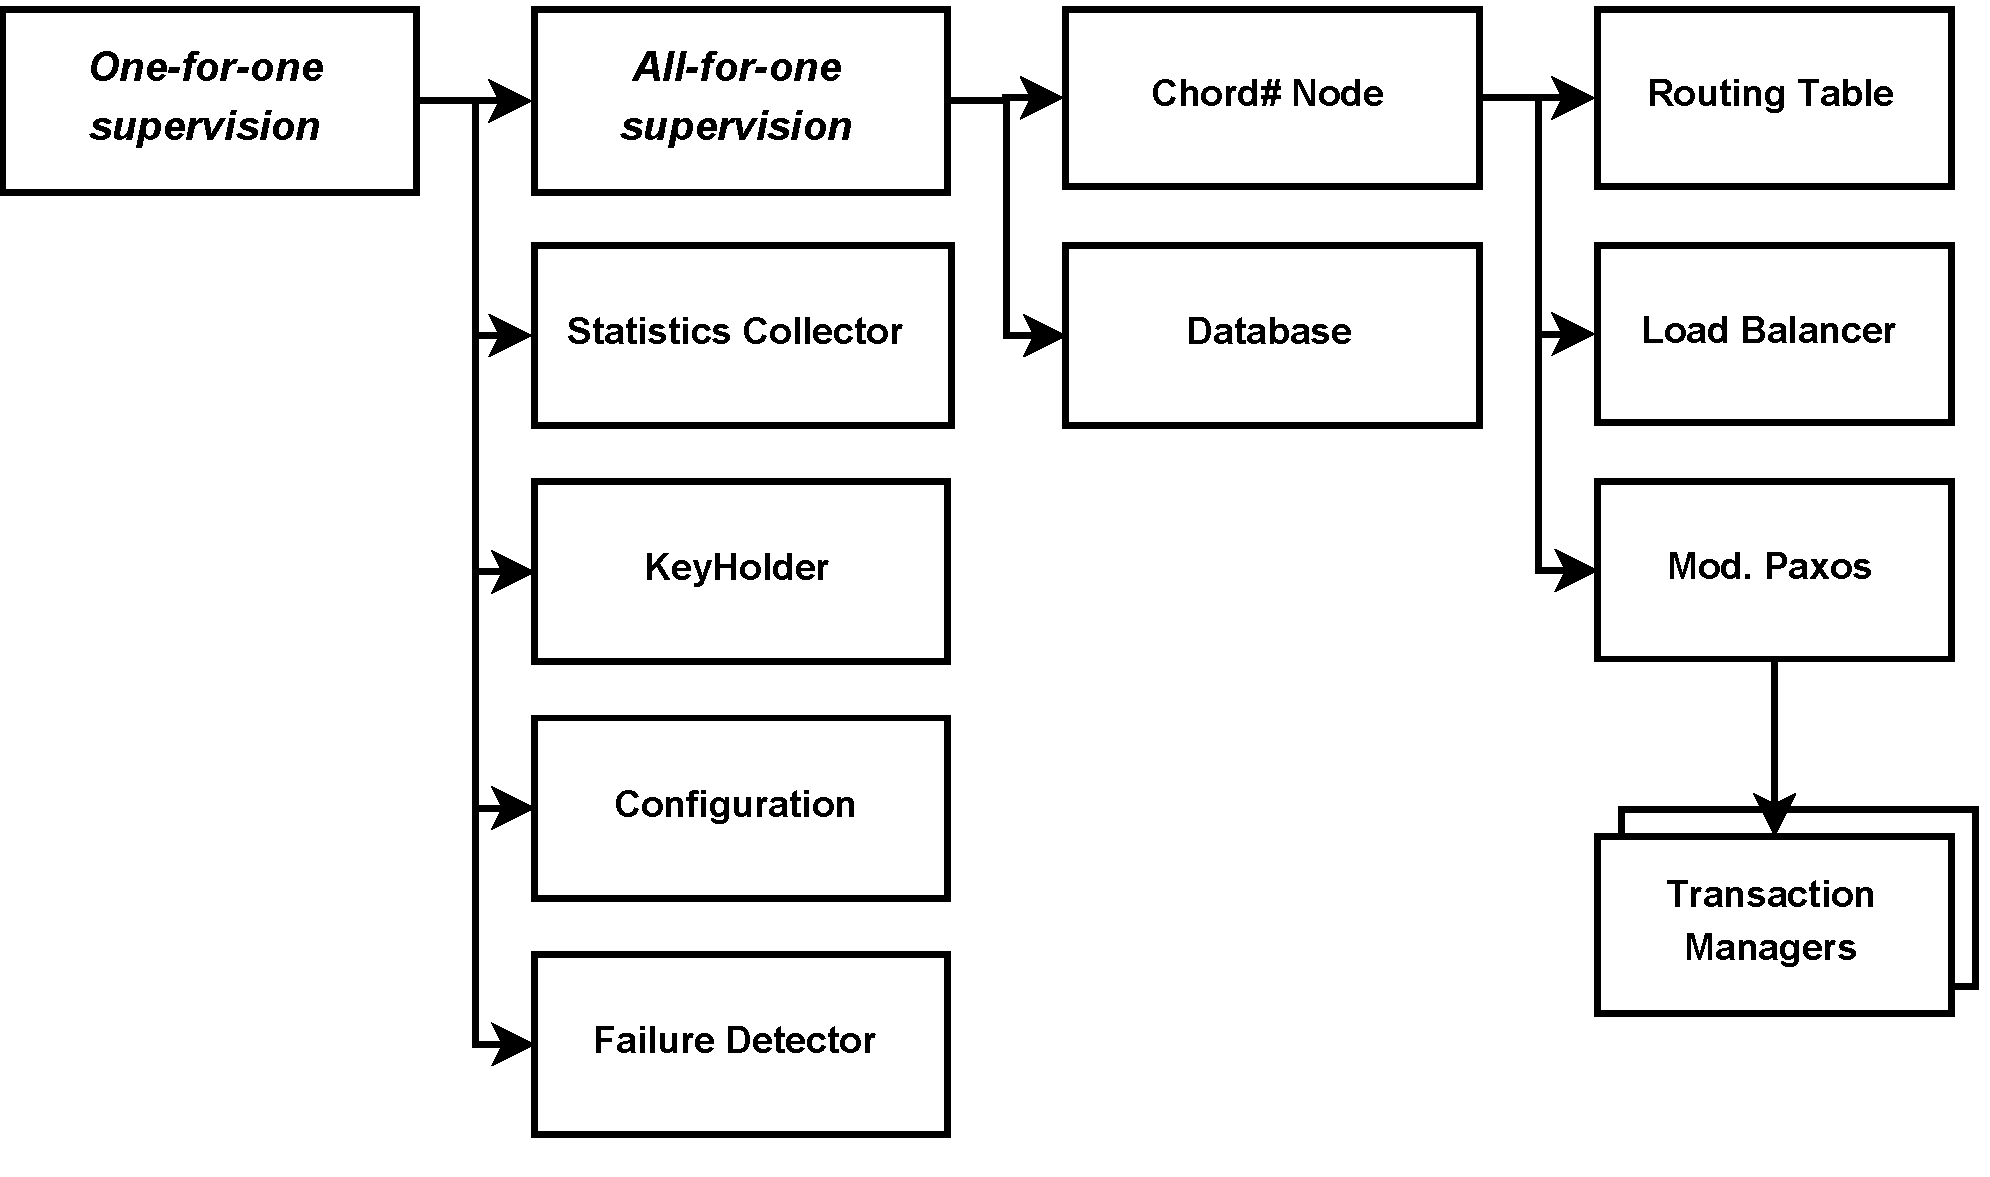
\includegraphics[width=\linewidth]{supervision}
\end{center}

When new nodes are started using \erlfun{admin}{add\_node}{/1}, only new
\code{sup_dht_node} supervisors are started.

\section{Starting the sup\_dht\_node supervisor and general processes of a node}

Starting supervisors is a two step process: a call to
\erlfun{supervisor}{start\_link}{/2,3}, e.g. from a custom supervisor's own
\code{start_link} method, will start the supervisor process. It will then
call \erlfun[]{Module}{init}{/1} to find out about the restart strategy,
maximum restart frequency and child processes.
Note that \erlfun{supervisor}{start\_link}{/2,3} will not return until
\erlfun[]{Module}{init}{/1} has returned and all child processes have been
started.

Let's have a look at \erlfun{sup\_dht\_node}{init}{/1}, the 'DHT node
supervisor'.

\codesnippet{sup_dht_node.erl}{sup_dht_node:init}{../src/sup_dht_node.erl}


The return value of the \code{init/1} function specifies the child
processes of the supervisor and how to start them. Here, we define a
list of processes to be observed by a \code{one_for_one}
supervisor. The processes are:
\code{Monitor},
\code{Delayer},
\code{Reregister},
\code{DeadNodeCache},
\code{RingMaintenance},
\code{RoutingTable},
\code{Cyclon},
\code{Vivaldi},
\code{DC_Clustering},
\code{Gossip} and a
\code{SupDHTNodeCore_AND} process in this order.

The term \code{\{one_for_one, 10, 1\}} specifies that the supervisor
should try 10 times to restart each process before giving
up. \code{one_for_one} supervision means, that if a single process
stops, only that process is restarted. The other processes run
independently.

When the \erlfun{sup\_dht\_node}{init}{/1} is finished the supervisor module
starts all the defined processes by calling the functions that were
defined in the returned list.

For a join of a new node, we are only interested in the starting of
the \code{SupDHTNodeCore_AND} process here. At that point in time, all
other defined processes are already started and running.

\section{Starting the sup\_dht\_node\_core supervisor with a peer and some paxos processes}

Like any other supervisor the \erlmodule{sup\_dht\_node\_core} supervisor
calls its \erlfun[]{sup\_dht\_node\_core}{init}{/1} function:

\codesnippet{sup_dht_node_core.erl}{sup_dht_node_core:init}{../src/sup_dht_node_core.erl}

It defines five processes, that have to be observed using a
\code{one_for_all}-supervisor, which means, that if one fails, all have to
be restarted. The \erlmodule{dht\_node} module implements the main
component of a full \scalaris{} node which glues together all the other
processes. Its
\erlfun[]{dht\_node}{start\_link}{/2} function will get
the following parameters: (a) the processes' group that is used with the \erlmodule{pid\_groups}
module and (b) a list of options for
the \erlmodule{dht\_node}. The process group name was calculated
a bit earlier in the code. \emph{Exercise: Try to find where.}


\codesnippet{dht_node.erl}{dht_node:start_link}{../src/dht_node.erl}

Like many other modules, the \erlmodule{dht\_node} module implements the
\code{gen_component}
behaviour. This behaviour was developed by us to enable us to write code which is
similar in syntax and semantics to the examples in~\cite{rachid-book}.
Similar to the \code{supervisor} behaviour, a module implementing this
behaviour has to
provide an \code{init/1} function, but here it is used to initialize the
state of the component. This function is described in the next
section.

Note: \code{?MODULE} is a predefined Erlang macro, which expands to the
module name, the code belongs to (here: \code{dht_node}).

\section{\texorpdfstring{Initializing a \code{dht_node}-process}
             {Initializing a dht\_node-process}}

\codesnippet{dht_node.erl}{dht_node:start}{../src/dht_node.erl}

The \code{gen_component} behaviour registers the \code{dht_node} in the
process dictionary. Formerly, the process had to do this itself, but
we moved this code into the behaviour. If an ID was given to
\erlfun{dht\_node}{init}{/1} function as a \code{\{\{dht_node, id\}, KEY\}}
tuple, the given Id will be used. Otherwise a random key is generated.
Depending on whether the node is the first inside a VM marked as first or not,
the according function in \erlmodule{dht\_node\_join} is called.
Also the pid of the node's supervisor is kept for future reference.

\section{Actually joining the ring}

After retrieving its identifier, the node starts the join protocol
which processes the appropriate messages calling
\erlfun{dht\_node\_join}{process\_join\_state}{Message, State}. On the
existing node, join messages will be processed by
\erlfun{dht\_node\_join}{process\_join\_msg}{Message, State}.

\subsection{A single node joining an empty ring}

\codesnippet{dht_node_join.erl}{dht_node_join:join_as_first}{../src/dht_node_join.erl}

If the ring is empty, the joining node will be the only node in the ring
and will thus be responsible for the whole key space.
It will trigger all known nodes to initialize the comm layer and then finish
the join.
\erlfun{dht\_node\_join}{finish\_join}{/5}
just creates a new state for a \scalaris{} node consisting of the given
parameters (the node as itself, its predecessor and successor,
an empty database and the queued messages that arrived during the join).
It then activates all dependent processes and creates a routing table from
this information.

The \erlfun{dht\_node\_state}{state}{} type is defined in

\codesnippet{dht_node_state.erl}{dht_node_state:state}{../src/dht_node_state.erl}

\subsection{A single node joining an existing (non-empty) ring}

If a node joins an existing ring, its join protocol will step through
the following four phases:
\begin{itemize}
  \item \makebox[4em][l]{\textbf{phase2}}
    finding nodes to contact with the help of the configured \code{known_hosts}
  \item \makebox[4em][l]{\textbf{phase2b}}
    getting the number of Ids to sample (may be skipped)
  \item \makebox[4em][l]{\textbf{phase3}}
    lookup nodes responsible for all sampled Ids
  \item \makebox[4em][l]{\textbf{phase4}}
    joining a selected node and setting up item movements
\end{itemize}

The following figure shows a (non-exhaustive) overview of the transitions
between the phases in the normal case. We will go through these step by step
and discuss what happens if errors occur.

\medskip
{\centering\documentclass[a4paper]{scrreprt}
\usepackage{typearea}
\areaset[1cm]{165mm}{240mm}

\usepackage[T1]{fontenc}
\usepackage[latin1]{inputenc}
\usepackage{listings}

\usepackage{xcolor}
\definecolor{lightyellow}{rgb}{1.0, 1.0, 0.5}
\definecolor{codebackground}{HTML}{EEEEEE}
\definecolor{commandinput}{rgb}{0.8,0.8,1}
\definecolor{lightblue}{HTML}{1E90FF}

\usepackage{tikz}
\usetikzlibrary{positioning}
\usetikzlibrary{shadows}
\usetikzlibrary{fit}
\usetikzlibrary{shapes.arrows}
\usetikzlibrary{backgrounds}
\usepackage[graphics,tightpage,active]{preview}
\PreviewEnvironment{tikzpicture}
\newlength{\imagewidth}
\newlength{\imagescale}

\usepackage{calc}

\newcommand{\code}[1]{\lstinline[basicstyle=\ttfamily]!#1!}

\begin{document}

% TODO: extend this picture and provide all paths between phases
\begin{tikzpicture}
 [rounded corners,
  pre/.style={<-,shorten <=1pt,>=stealth,semithick},
  post/.style={->,shorten >=1pt,>=stealth,semithick},
  timeout/.style={draw=black!50, dashed},
  phase/.style={rectangle,top color=black!10,bottom color=black!5},
  bend angle=60]
 \node[phase] (phase1)                         {init};
 \node[phase] (phase2)  [right=3.5 of phase1]  {phase2};
 \node[phase] (phase2b) [below=3 of phase2]    {phase2b};
 \node[phase] (phase3)  [right=3.5 of phase2]  {phase3};
 \node[phase] (phase4)  [right=3.5 of phase3]  {phase4};


 \path[->] (phase2)
             edge [pre]  node[auto, swap] {get\_known\_nodes()} (phase1)
             edge [post] node[auto, swap, align=right]
                          {
                           get\_number\_of\_samples()\\
                           \footnotesize{\textcolor{red}{skip\_psv\_lb not set,}}\\
                           \footnotesize{\textcolor{red}{non-empty ContactNodes}}
                          } (phase2b)
             edge [post] node[auto, align=left, pos=0.475]
                          {
                           lookup\_new\_ids2()\\
                           ~\footnotesize{$\hookrightarrow$lookup\_new\_ids1()}\\
                           ~~\scriptsize{$\hookrightarrow$lookup()}
                          }
                         node[auto, swap, align=left, pos=0.525]
                          {
                           \footnotesize{\textcolor{red}{skip\_psv\_lb set,}}\\
                           \footnotesize{\textcolor{red}{non-empty ContactNodes}}
                          } (phase3)
           (phase2b)
             edge [post, bend left=-35]
                         node[auto, swap, pos=0.6, align=left]
                          {
                           lookup\_new\_ids2()\\
                           ~\footnotesize{$\hookrightarrow$lookup\_new\_ids1()}\\
                           ~~\scriptsize{$\hookrightarrow$lookup()}\\
                          } (phase3)
           (phase3)
             edge [post] node[auto, align=center, pos=0.5]
                          {
                           contact\_best\_candidate()\\
                           \footnotesize{$\hookrightarrow$ send\_join\_request()}
                          } (phase4);
\end{tikzpicture}
\end{document}

}

At first all nodes set in the \code{known_hosts} configuration parameter are
contacted. Their responses are then handled in phase~2. In order to separate
the join state from the ordinary \code{dht_node} state, the
\code{gen_component} is instructed to use the \erlfun{dht\_node}{on\_join}{/2}
message handler which delegates every message to
\erlfun{dht\_node\_join}{process\_join\_state}{/2}.

\codesnippet{dht_node_join.erl}{dht_node_join:join_as_other}{../src/dht_node_join.erl}

\subsubsection{Phase 2 and 2b}

Phase~2 collects all \erlmodule{dht\_node} processes inside the contacted
VMs. It therefore mainly processes \code{get_dht_nodes_response} messages and
integrates all received nodes into the list of available connections.
The next step depends on whether the \code{\{skip_psv_lb\}} option for
skipping any passive load balancing algorithm has been
given to the \erlmodule{dht\_node} or not. If it is present, the node will
only use the ID that has been initially passed to
\erlfun{dht\_node\_join}{join\_as\_other}{/3}, issue a lookup for the
responsible
node and move to phase~3. Otherwise, the passive load balancing's
\erlfun{lb\_psv\_*}{get\_number\_of\_samples}{/1} method will be called
asking for the number of IDs to sample. Its answer will be processed in
phase~2b.

\code{get_dht_nodes_response} messages arriving in phase~2b or later will be
processed anyway and received \erlmodule{dht\_node}
processes will be integrated into the connections. These phases'
operations will not be interrupted and nothing else is changed though.

\codesnippet{dht_node_join.erl}{dht_node_join:join_other_p2}{../src/dht_node_join.erl}

Phase~2b will handle \code{get_number_of_samples} messages from the passive
load balance algorithm. Once received, new (unique) IDs will be sampled
randomly so that the total number of join candidates (selected IDs together
with fully processed candidates from further phases) is at least as high as
the given number of samples. Afterwards, lookups will be created for all
previous IDs as well as the new ones and the node will move to phase~3.

\codesnippet{dht_node_join.erl}{dht_node_join:join_other_p2b}{../src/dht_node_join.erl}

Lookups will make \scalaris{} find the node currently responsible for a given ID
and send a request to simulate a join to this node, i.e. a
\code{get_candidate} message. Note that during such an operation, the joining
node would become the existing node's predecessor. The simulation will be
delegated to the passive load balance algorithm the joining node requested, as
set by the \code{join_lb_psv} configuration parameter. 

\codesnippet{dht_node_join.erl}{dht_node_join:get_candidate}{../src/dht_node_join.erl}

\subsubsection{Phase 3}

The result of the simulation will be send in a \code{get_candidate_response}
message and will be processed in phase~3 of the joining node. It will be
integrated into the list of processed candidates. If there are no more IDs
left to process, the best among them will be contacted. Otherwise further
\code{get_candidate_response} messages will be awaited.
Such messages will also be processed in the other phases where the candidate
will be simply added to the list.

\codesnippet{dht_node_join.erl}{dht_node_join:join_other_p3}{../src/dht_node_join.erl}

If \erlfun{dht\_node\_join}{contact\_best\_candidate}{/1} is called and
candidates are available (there should be at this stage!), it will sort the
candidates by using the passive load balance algorithm, send a 
\code{join_request} message and continue with phase~4. 

\erlfunindex{dht\_node\_join}{contact\_best\_candidate}
\codesnippet{dht_node_join.erl}{dht_node_join:contact_best_candidate}{../src/dht_node_join.erl}
\erlfunindex{dht\_node\_join}{send\_join\_request}
\codesnippet{dht_node_join.erl}{dht_node_join:send_join_request}{../src/dht_node_join.erl}

The \code{join_request} message will be received by the existing node which
will set up a slide operation with the new node. If it is not responsible for
the key (anymore), it will deny the request and reply with a
\code{\{join, join_response, not_responsible, Node\}} message.
If it is responsible for the ID and is not participating in a slide with its
current predecessor, it will set up a slide with the joining node:

\codesnippet{dht_node_join.erl}{dht_node_join:join_request1}{../src/dht_node_join.erl}

\subsubsection{Phase 4}

The joining node will receive the \code{join_response} message in phase~4 of
the join protocol. If everything is ok, it will
notify its ring maintenance process that it enters the ring, start all required
processes and join the slide operation set up by the existing node in order to
receive some of its data.

If the join candidate's node is not responsible for the candidate's ID anymore
or the candidate's ID already exists, the next candidate is contacted until
no further candidates are available and the join protocol starts over using
\erlfun{dht\_node\_join}{start\_over}{/1}.

Note that the \code{join_response} message will actually be processed in
any phase. Therefore, if messages arrive late, the join can be processed
immediately and the rest of the join protocol does not need to be executed
again.

\codesnippet{dht_node_join.erl}{dht_node_join:join_other_p4}{../src/dht_node_join.erl}
\erlfunindex{dht\_node\_join}{finish\_join}
\erlfunindex{dht\_node\_join}{finish\_join\_and\_slide}
\codesnippet{dht_node_join.erl}{dht_node_join:finish_join}{../src/dht_node_join.erl}

The macro \code{?RT} maps to the configured routing algorithm. It is defined
in \code{include/scalaris.hrl}. For further details on the routing see
Chapter~\sieheref{chapter.routing}.

\subsubsection{Timeouts and other errors}

The following table summarizes the timeout messages send during the join
protocol on the joining node. It shows in which of the phases each of the
messages is processed and describes (in short) what actions are taken.
All of these messages are influenced by their respective config parameters,
e.g. \code{join_timeout} parameter in the config files defines an overall
timeout for the whole join operation. If it takes longer than
\code{join_timeout} ms, a \code{\{join, timeout\}} will be send and processed
as given in this table.

\medskip
{\small
\begin{tabular}{lP{2.4cm}P{2.75cm}P{2.35cm}P{3.25cm}M{1.70cm}}
  \toprule
  & \code{known_hosts}\carriagereturn\newline\code{_timeout}
  & \code{get_number_of}\carriagereturn\newline\code{_samples}\carriagereturn\newline\code{_timeout}
  & \code{lookup}\carriagereturn\newline\code{ _timeout}
  & \code{join_request}\carriagereturn\newline\code{_timeout}
  & \code{timeout} \tn
  \midrule
  %
  \bfseries phase2
  & get known nodes from configured VMs
  & ignore
  & ignore
  & ignore
  & \multirow{21}{1.70cm}
        {re-start join\newline$\rightarrow$ phase~2 or 2b} \tn
  \cmidrule(r){1-5}
  %
  \bfseries phase2b
  & ignore
  & remove contact node, re-start join\newline
    $\rightarrow$ phase~2 or 2b
  & ignore
  & ignore
  & \tn
  \cmidrule(r){1-5}
  %
  \bfseries phase3
  & ignore
  & ignore
  & remove contact node, lookup remaining IDs\newline
    $\rightarrow$ phase~2 or 3 
  & ignore
  & \tn
  \cmidrule(r){1-5}
  %
  \bfseries phase3b
  & ignore
  & ignore
  & ignore
  & ignore
  & \tn
  \cmidrule(r){1-5}
  %
  \bfseries phase4
  & ignore
  & ignore
  & ignore
  & timeouts $< 3$?\footnote{set by the \code{join_request_timeouts} config parameter}\newline
    \mbox{}~$\rightarrow$ contact candidate\newline
    otherwise:\newline
    \mbox{}~remove candidate\newline
    \mbox{}~no candidates left?\newline
    \mbox{}~~$\rightarrow$ phase~2 or 2b\newline
    \mbox{}~otherwise:\newline
    \mbox{}~~$\rightarrow$ contact next one\newline
    \mbox{}~~$\rightarrow$ phase~3b or 4
  & \tn
  \bottomrule
\end{tabular}
}
\medskip

On the existing node, there is only one timeout message which is part of the
join protocol: the \code{join_response_timeout}. It will be send when a slide
operation is set up and if the timeout hits before the next message exchange,
it will increase the slide operation's number of timeouts. The slide will be
aborted if at least \code{join_response_timeouts} timeouts have been received.
This parameter is set in the config file.

\subsubsection{Misc. (all phases)}

Note that join-related messages arriving in other phases than those handling
them will be ignored. Any other messages during a \code{dht_node}'s join will
be queued and re-send when the join is complete.
